%!TEX TS-program = xelatex
%!TEX encoding = UTF-8 Unicode
\documentclass{beamer}
\usepackage{amsmath, amsthm, amssymb}
\usepackage[no-math]{fontspec}
\usepackage{xeCJK}
\usepackage{pstricks-add}

\setCJKmainfont{WenQuanYi Micro Hei}
\hypersetup{colorlinks, linkcolor=, unicode}
\useoutertheme{sidebar}
\usecolortheme{rose}
\usecolortheme{seahorse}

\renewcommand{\today}{\number\year~年 \number\month~月 \number\day~日}

\logo{\href{https://github.com/jdh8/calculus-slides}{
\includegraphics[scale=1.6]{include/favicon.eps}}}

\author[何震邦]{
    何震邦 \href{http://jdh8.org/}{<jdh8.org>} \\[1ex]
    \href{https://creativecommons.org/licenses/by-sa/4.0/deed.zh_TW}{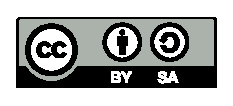
\includegraphics{include/by-sa.eps}}
}


\begin{document}
\title[微積分演習課]{\href{https://jdh8.github.io/calculus-slides/Introduction.pdf}{臺北醫學大學微積分演習課}}
\maketitle

\section{前言}
\begin{frame}{關於我}
    \begin{columns}[onlytextwidth]
        \begin{column}{0.6\textwidth}
            \begin{itemize}
                \item \href{http://my2.tmu.edu.tw/b101100025}{B101100025}
                \item \href{https://www.facebook.com/jdh863}{臉書}
                \item \href{https://plus.google.com/+\%E4\%BD\%95\%E9\%9C\%87\%E9\%82\%A6-jdh8}{Google+}
                \item 0918-319823
                    \begin{itemize}
                        \item 真是充滿火藥味的號碼
                    \end{itemize}
            \end{itemize}
        \end{column}

        \begin{column}{0.4\textwidth}
            \begin{flushleft}
                \newlength{\stickerwidth}
                \setlength{\stickerwidth}{\columnwidth - 1em}
                
\includegraphics[width=\stickerwidth]{Introduction/sticker.jpg}
            \end{flushleft}
        \end{column}
    \end{columns}
\end{frame}

\begin{frame}{課程內容}
    以培養解題能力為目標。先通過考試,後培養邏輯思辨能力。

    \begin{itemize}
        \item \href{https://jdh8.github.io/calculus-slides/}{投影片}
        \item \href{http://jdh8.org/category/calculus-course/}{考古題、上課影片}
        \item 網頁教材(建構中)
            \begin{itemize}
                \item \href{http://jdh8.org/calculus/}{部落格頁面}
                \item \href{https://zh.wikibooks.org/wiki/\%E5\%BE\%AE\%E7\%A7\%AF\%E5\%88\%86\%E5\%AD\%A6}{維基教科書}
            \end{itemize}
    \end{itemize}
\end{frame}
\end{document}
